% !TeX root = ../../../main.tex
\subsection{Medication Subgroup Analysis}\ChThreeHeadingOnly
\label{ch03:apd:medication_subgroup_analysis}





\subsubsection{Individual Treatment Effect for Medication Types}
\label{ch03:apd:ite_medication}


% !TeX root = ../../../main.tex
\begin{figure}[htbp]
\ChThreeFloatContents
  {ch03:fig:ite_medication}
  {\caption{Distribution of Estimated Individual Treatment Effects (ITE) for the top four medications—\textcolor{blue}{risperidone}, \textcolor{orange}{aripiprazole}, \textcolor{ChThreeForestGreen}{olanzapine}, and \textcolor{red}{haloperidol}—evaluated using different survival models and T-learner at time snapshot \(\tau=3\) month. 
  The mean treatment effect (ATE) for each medication is provided in the legend.
  (a)-(c) show T-learner ITEs for (a) CoxPH, (b) DeepSurv, (c) Random Survival Forest. 
  (d) shows the ITE for Causal Survival Forest}}
  {%
    \subfigure[\footnotesize (CoxPH, T-Learner)]{\label{ch03:fig:ite_medication_coxph}%
      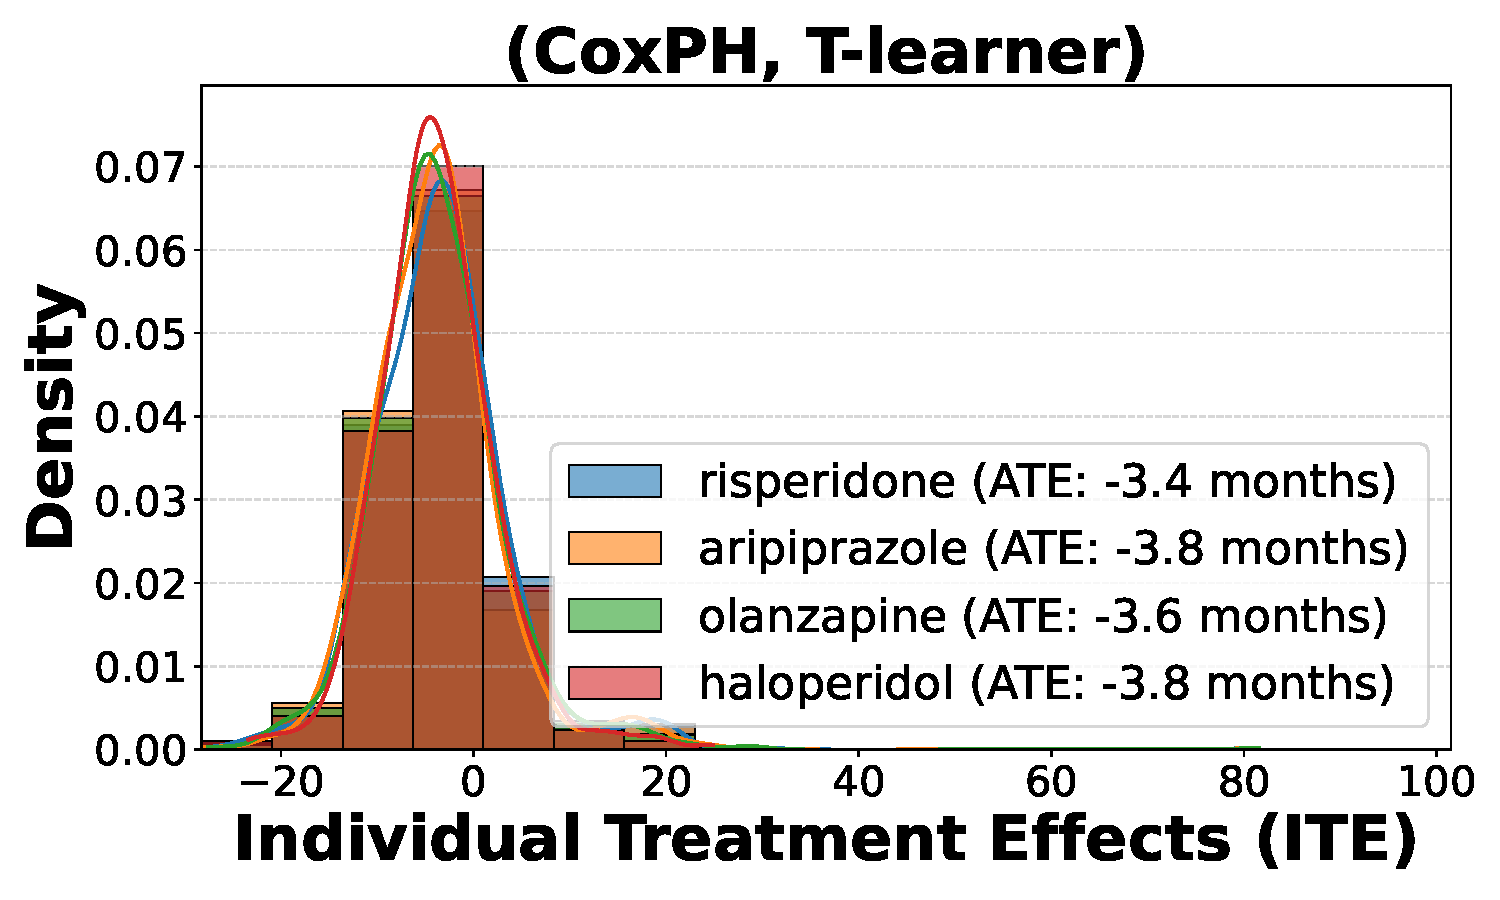
\includegraphics[width=.22\linewidth]{Appendices/appendix-ch03/images/ITE_medication/ITE_CoxPH_T-learner_med_type.pdf}}%
    \hfill
    \subfigure[\footnotesize (DeepSurv, T-Learner)]{\label{ch03:fig:ite_medication_deepsurv}%
      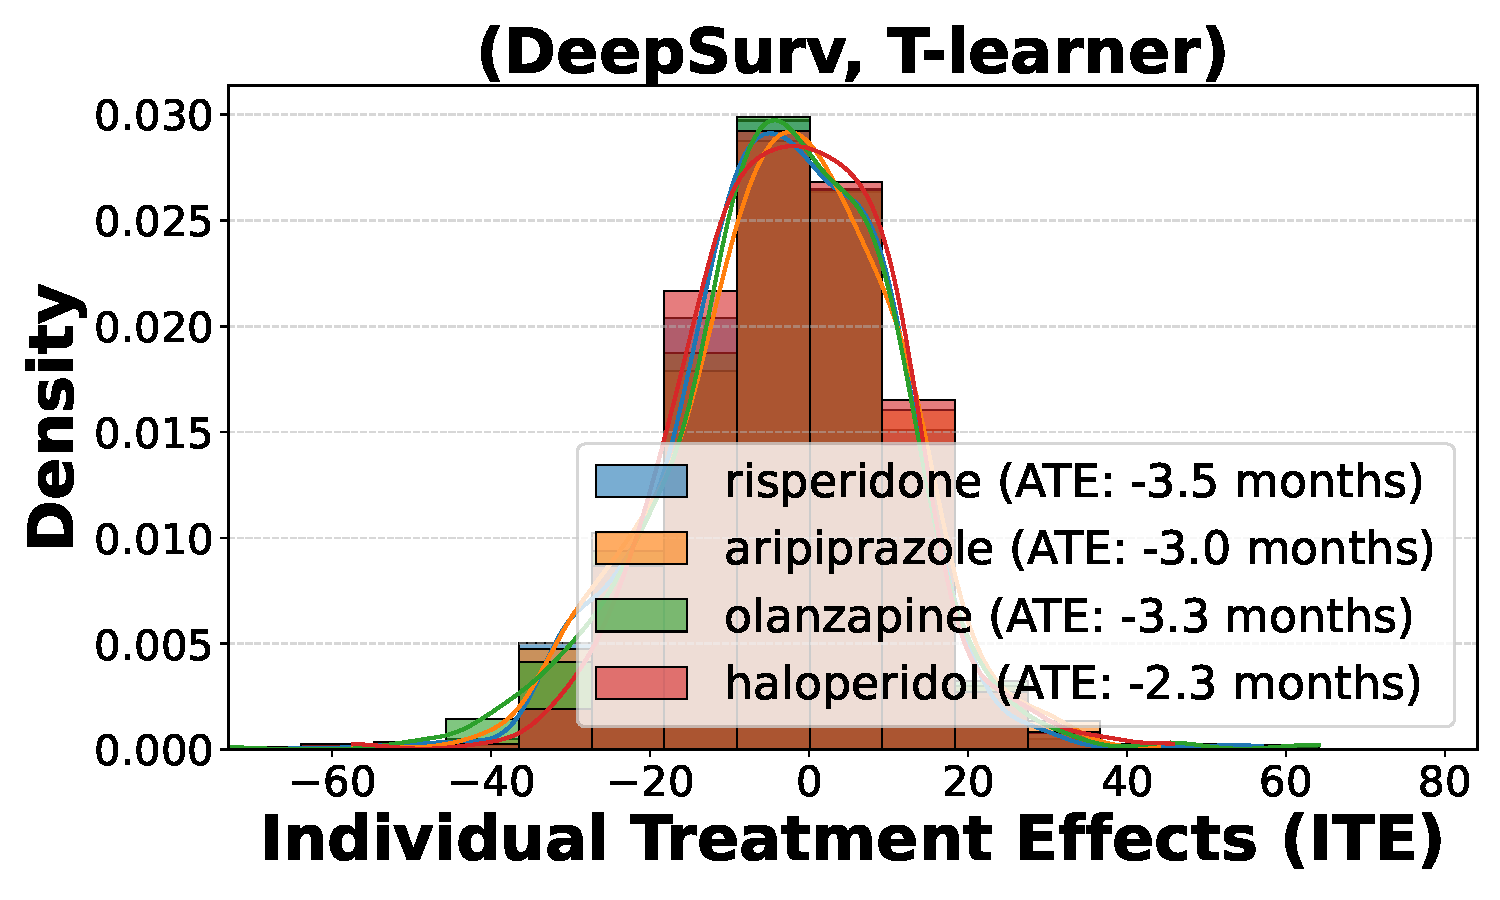
\includegraphics[width=.22\linewidth]{Appendices/appendix-ch03/images/ITE_medication/ITE_DeepSurv_T-learner_med_type.pdf}}%
    \hfill
    \subfigure[\footnotesize (RandomSurvivalForest, T-Learner)]{\label{ch03:fig:ite_medication_random_survival_forest}%
      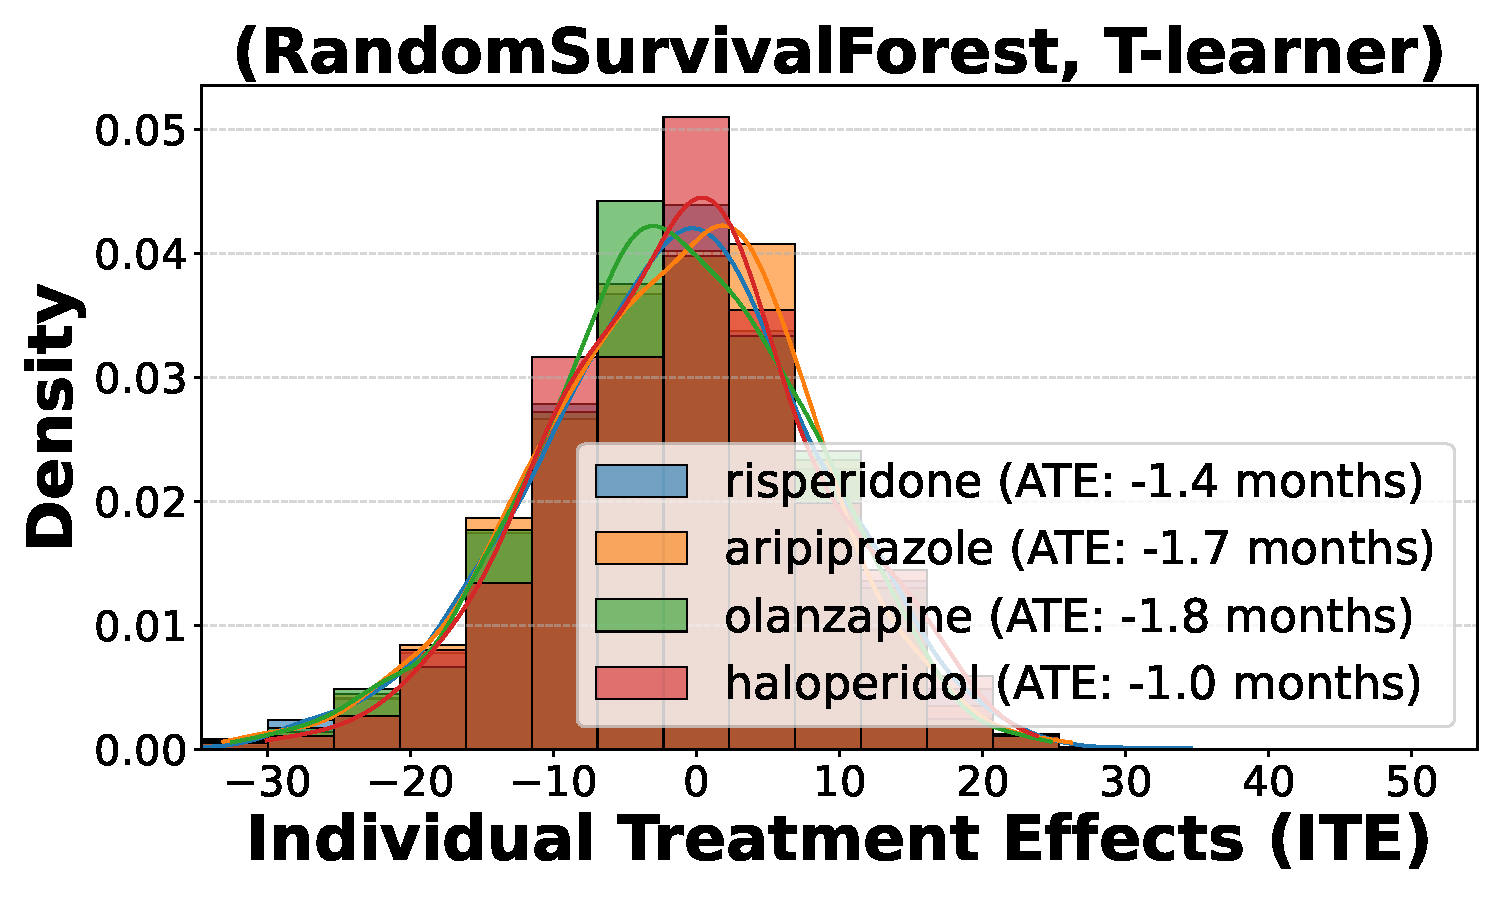
\includegraphics[width=.22\linewidth]{Appendices/appendix-ch03/images/ITE_medication/ITE_RandomSurvivalForest_T-learner_med_type.pdf}}%
    \hfill
    \subfigure[\footnotesize CausalSurvivalForest]{\label{ch03:fig:ite_medical_causal_survival_forest}%
      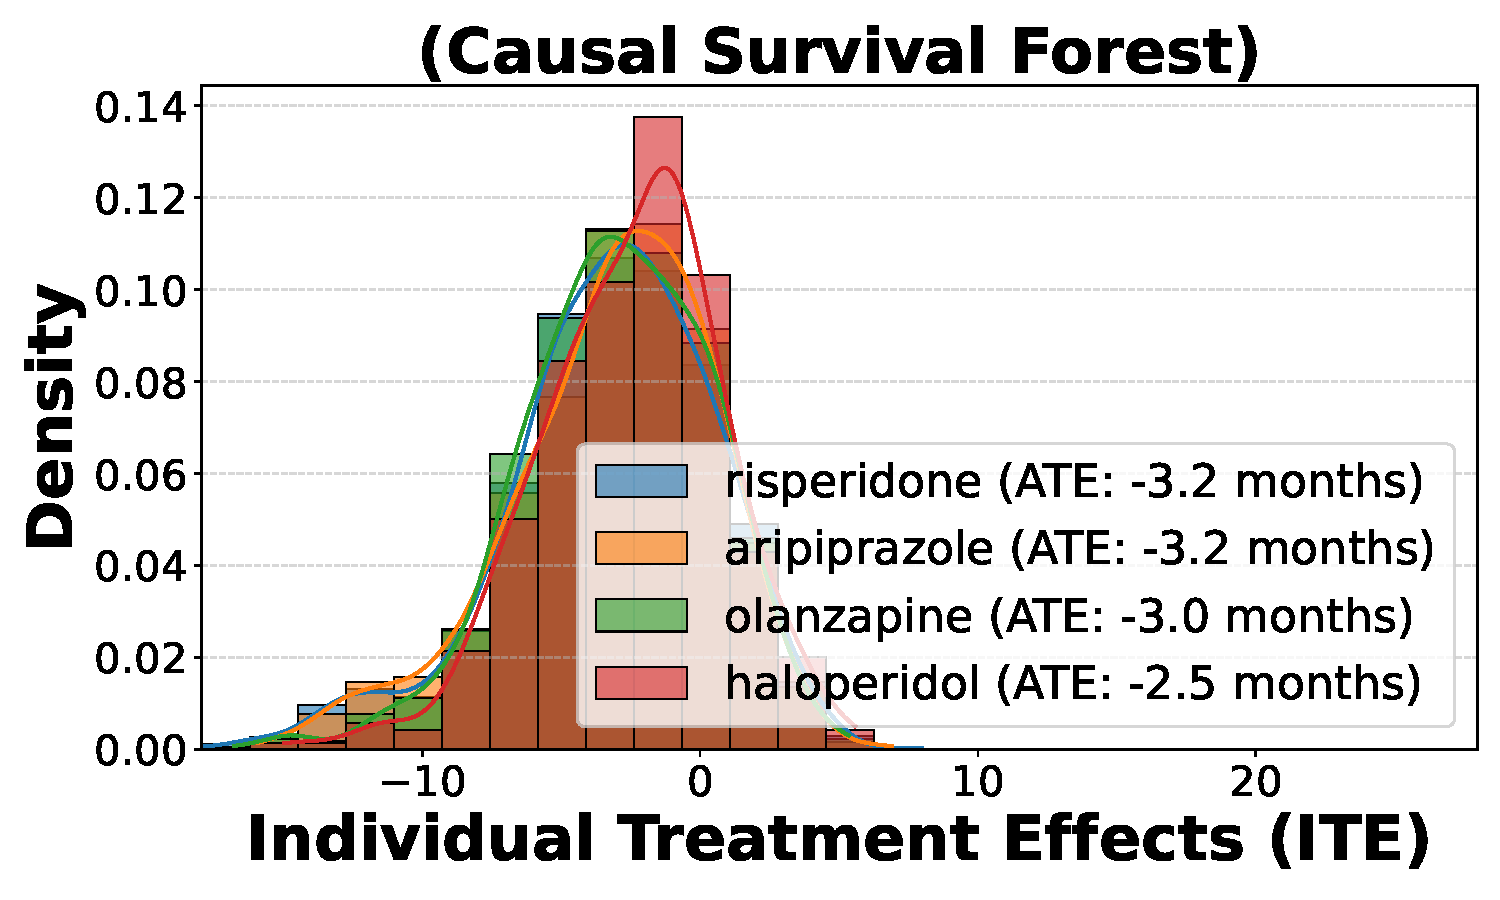
\includegraphics[width=.21\linewidth]{Appendices/appendix-ch03/images/ITE_medication/ITE_CausalSurvivalForest_Causal_Survival_Forest_med_type.pdf}}%
  }
\end{figure}


This section presents the distributions of Estimated Individual Treatment Effects (ITE) for the four most prevalent antipsychotic medications—risperidone, aripiprazole, olanzapine, and haloperidol—evaluated using various survival models and meta-learners.

Figure~\ref{ch03:fig:ite_medication} shows the ITE distributions at the time snapshot \(\tau=3\) months.
The plots compare the results from (a) Cox Proportional Hazards (CoxPH) model with T-learner, (b) DeepSurv with T-learner, (c) Random Survival Forest (RSF) with T-learner, and (d) Causal Survival Forest (CSF).
Each histogram is overlaid with a kernel density estimate to visualize the distribution shapes better.
The legend provides the average treatment effect (ATE) for each medication.

From Figure~\ref{ch03:fig:ite_medication}, the Causal Survival Forest (Figure~\ref{ch03:fig:ite_medical_causal_survival_forest}) produces the narrowest ITE distributions, indicating reduced variability and more consistent estimates compared to other models. 
The Random Survival Forest (Figure~\ref{ch03:fig:ite_medication_random_survival_forest}) shows slightly wider ITE distributions compared to the Causal Survival Forest but narrower distributions than the CoxPH (Figure~\ref{ch03:fig:ite_medication_coxph}) and DeepSurv (Figure~\ref{ch03:fig:ite_medication_deepsurv}) models, which exhibit the broadest ITE variability.

The ATE values across models exhibit different patterns and rankings for the medications. 
For CoxPH, haloperidol and aripiprazole share the most negative ATE values (\(-3.8\) months), followed by olanzapine (\(-3.6\)) and risperidone (\(-3.4\)). 
DeepSurv assigns the most negative ATE to risperidone (\(-3.5\)), followed by olanzapine (\(-3.3\)), aripiprazole (\(-3.0\)), and haloperidol (\(-2.3\)). 
In contrast, Random Survival Forest shows markedly smaller magnitude for all ATEs, with olanzapine (\(-1.8\)) being the most negative, followed by aripiprazole (\(-1.7\)), risperidone (\(-1.4\)), and haloperidol (\(-1.0\)). 
The Causal Survival Forest shows a pattern where risperidone and aripiprazole are tied at \(-3.2\), followed by olanzapine (\(-3.0\)) and haloperidol (\(-2.5\)).

These slight differences highlight that the ATE values for each medication within a given model are very similar, indicating no meaningful differences in treatment effects across the four most prevalent medications in our data.
While the ranking of ATEs for the medications varies slightly across models, the magnitudes are close within each model, further emphasizing the lack of significant differences among medications for any specific survival model. 
Additionally, we observe variability in ATE estimates across different models. 
The ATEs estimated by CoxPH, DeepSurv, and the Causal Survival Forest are closer to each other in magnitude, while the Random Survival Forest produces shorter ATE estimates compared to the other models. 
Another noteworthy observation is that the ATEs are consistently negative across all medications and models, which agrees with our previous results in Section~\ref{ch03:sec:experiments_results}, demonstrating shorter adverse event times for non-adherence regardless of the specific medication. 
This consistency in negative ATEs highlights the robustness of the association between non-adherence and reduced adverse event time in our analysis across the most prevalent antipsychotic medications.

\subsubsection{Individual Treatment Effects for Different Antipsychotic Administration Type}
\label{ch03:apd:ite_injectable_all}



% !TeX root = ../../../main.tex
\begin{figure}[!ht]
\ChThreeFloatContents
  {ch03:fig:ite_injectable_all}
  { \caption{
  Distribution of Estimated Individual Treatment Effects (ITE) for different medication adherence groups: \textcolor{ChThreeForestGreen}{injectable}, \textcolor{orange}{non-injectable}, and \textcolor{purple}{not covered} at time snapshot \(\tau=3\) months. 
  Each plot's legend highlights the Average Treatment Effect (ATE) in months for the groups covered by \textcolor{ChThreeForestGreen}{injectable} medication, \textcolor{orange}{non-injectable} medication, and those \textcolor{purple}{not covered} by any medication.
  (a)-(d) Show CoxPH survival model paired with various causal methods.
  (e)-(h) Show DeepSurv survival model paired with various causal methods.
  (i)-(l) Show Random Survival Forest paired with various causal methods.
  (m) shows Causal Survival Forest.
  Causal methods across each column is T-learner, S-learner, Matching method with 1 match, and Matching method with 5 matches.}}
  {%
    \subfigure[\footnotesize (CoxPH, T-Learner)]{\label{ch03:fig:ite_injectable_coxph_t_learner}%
      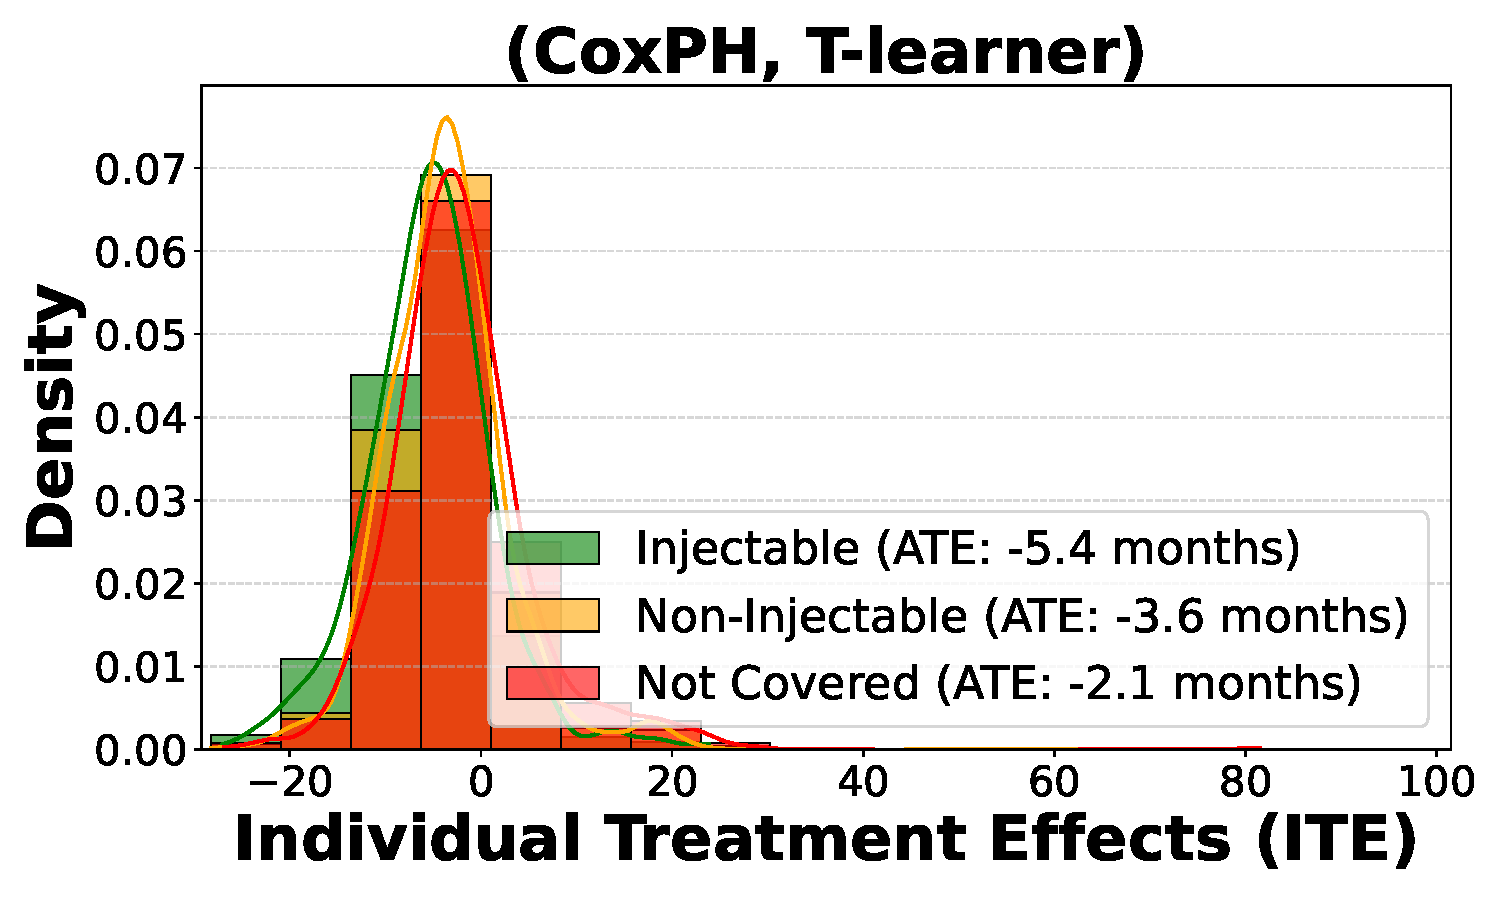
\includegraphics[width=.22\linewidth]{Appendices/appendix-ch03/images/ITE_injectable_full_3/ITE_CoxPH_T-learner_injectable_type.pdf}}%
    \hfill
    \subfigure[\footnotesize (CoxPH, S-Learner)]{\label{ch03:fig:ite_injectable_coxph_s_learner}%
      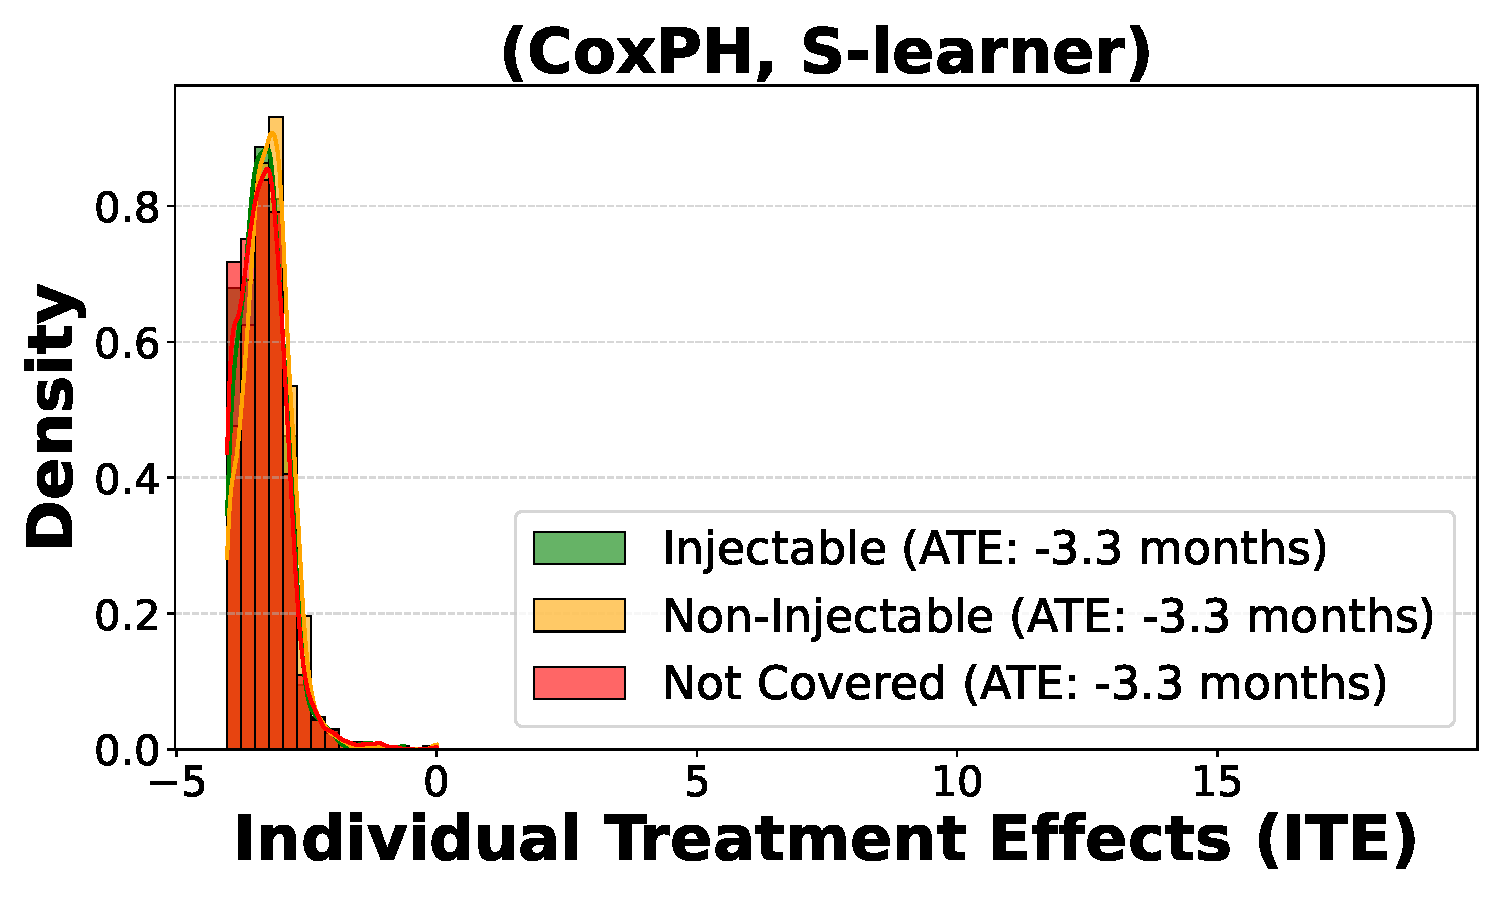
\includegraphics[width=.22\linewidth]{Appendices/appendix-ch03/images/ITE_injectable_full_3/ITE_CoxPH_S-learner_injectable_type.pdf}}%
    \hfill
    \subfigure[\footnotesize (CoxPH, Matching-1)]{\label{ch03:fig:ite_injectable_coxph_matching_1}%
      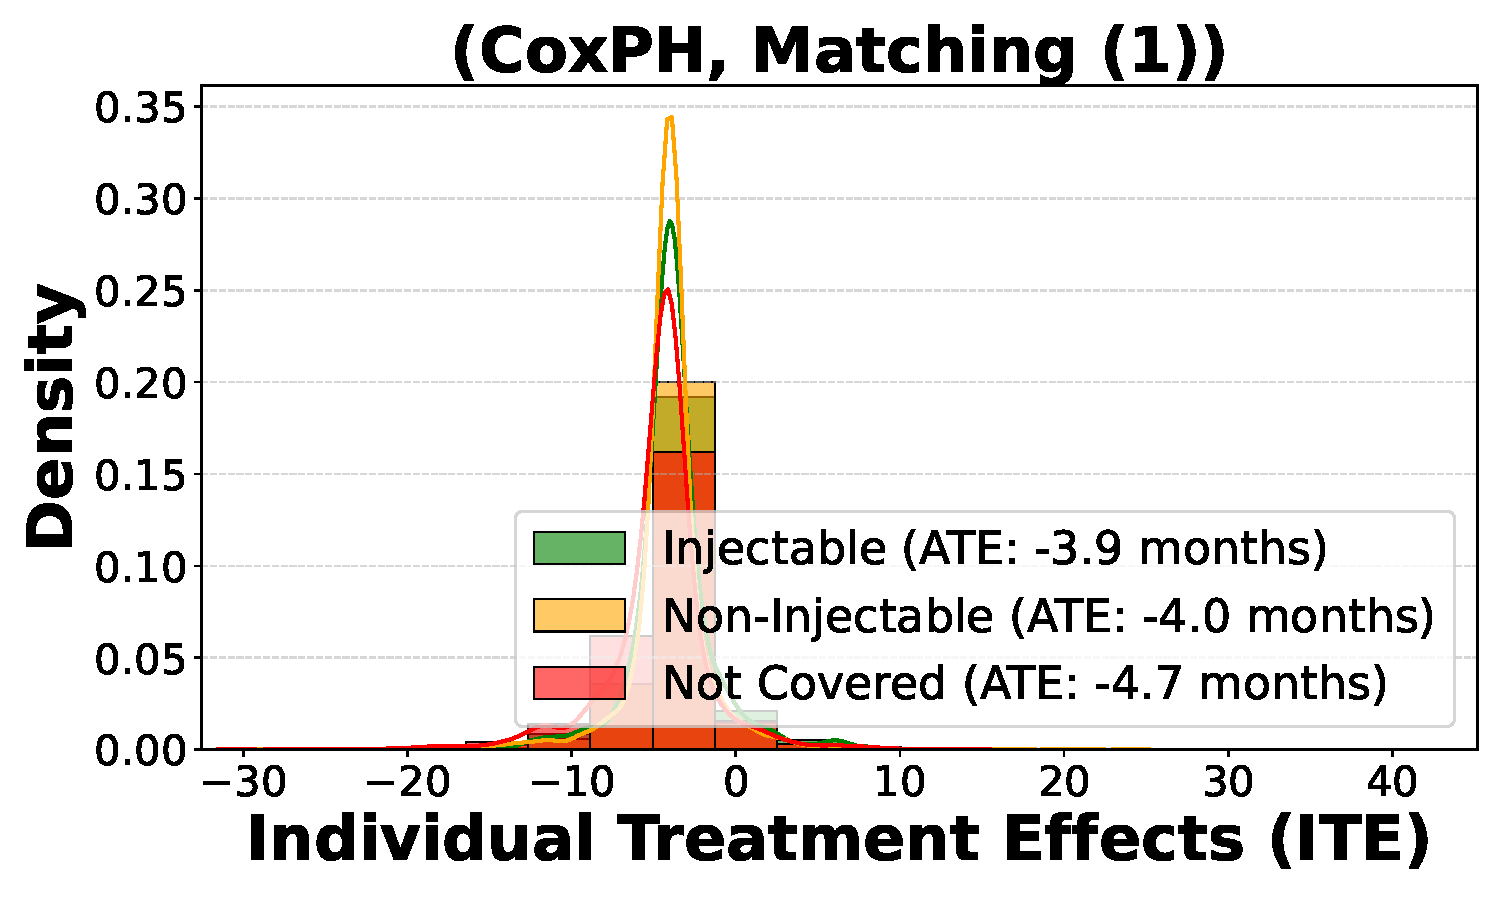
\includegraphics[width=.22\linewidth]{Appendices/appendix-ch03/images/ITE_injectable_full_3/ITE_CoxPH_Matching_1_injectable_type.pdf}}%
    \hfill
    \subfigure[\footnotesize (CoxPH, Matching-5)]{\label{ch03:fig:ite_injectable_coxph_matching_5}%
      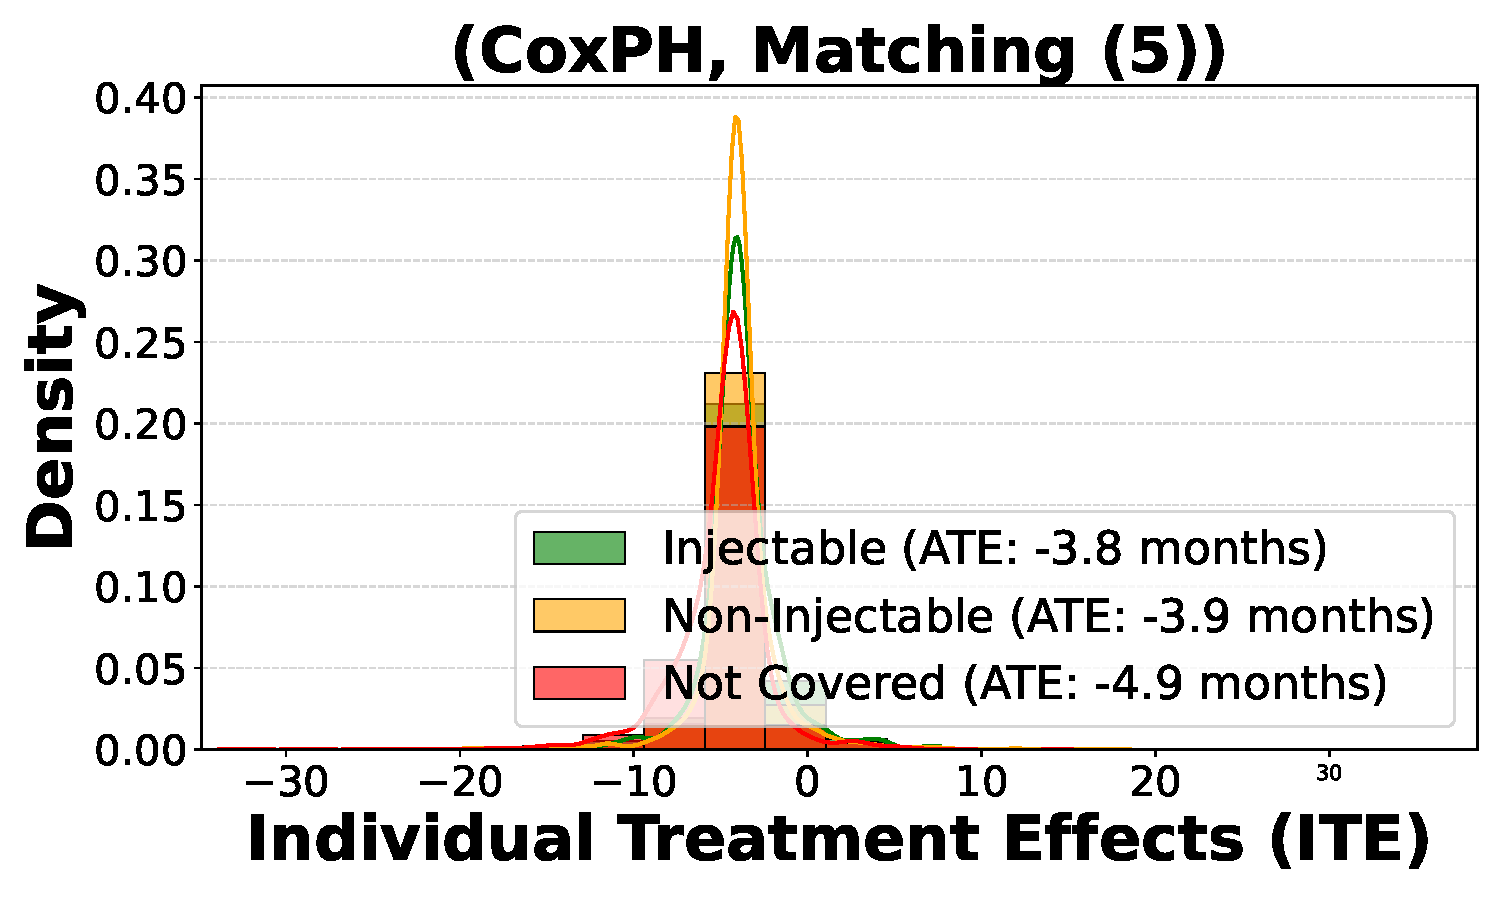
\includegraphics[width=.21\linewidth]{Appendices/appendix-ch03/images/ITE_injectable_full_3/ITE_CoxPH_Matching_5_injectable_type.pdf}}%
    \\
    \subfigure[\footnotesize (DeepSurv, T-Learner)]{\label{ch03:fig:ite_injectable_deepsurv_t_learner}%
      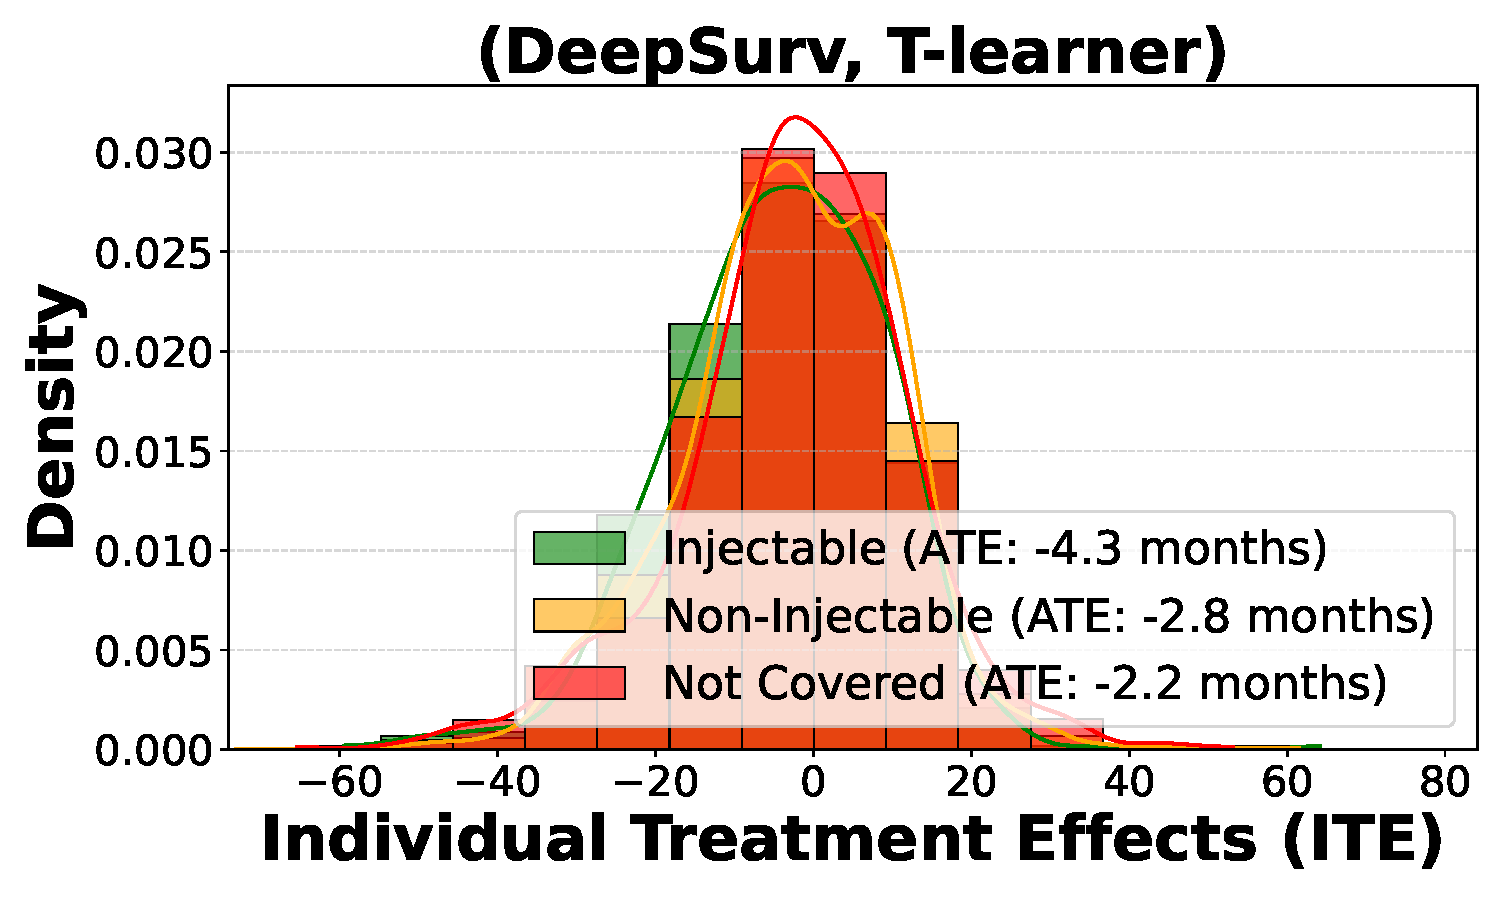
\includegraphics[width=.22\linewidth]{Appendices/appendix-ch03/images/ITE_injectable_full_3/ITE_DeepSurv_T-learner_injectable_type.pdf}}%
    \hfill
    \subfigure[\footnotesize (DeepSurv, S-Learner)]{\label{ch03:fig:ite_injectable_deepsurv_s_learner}%
      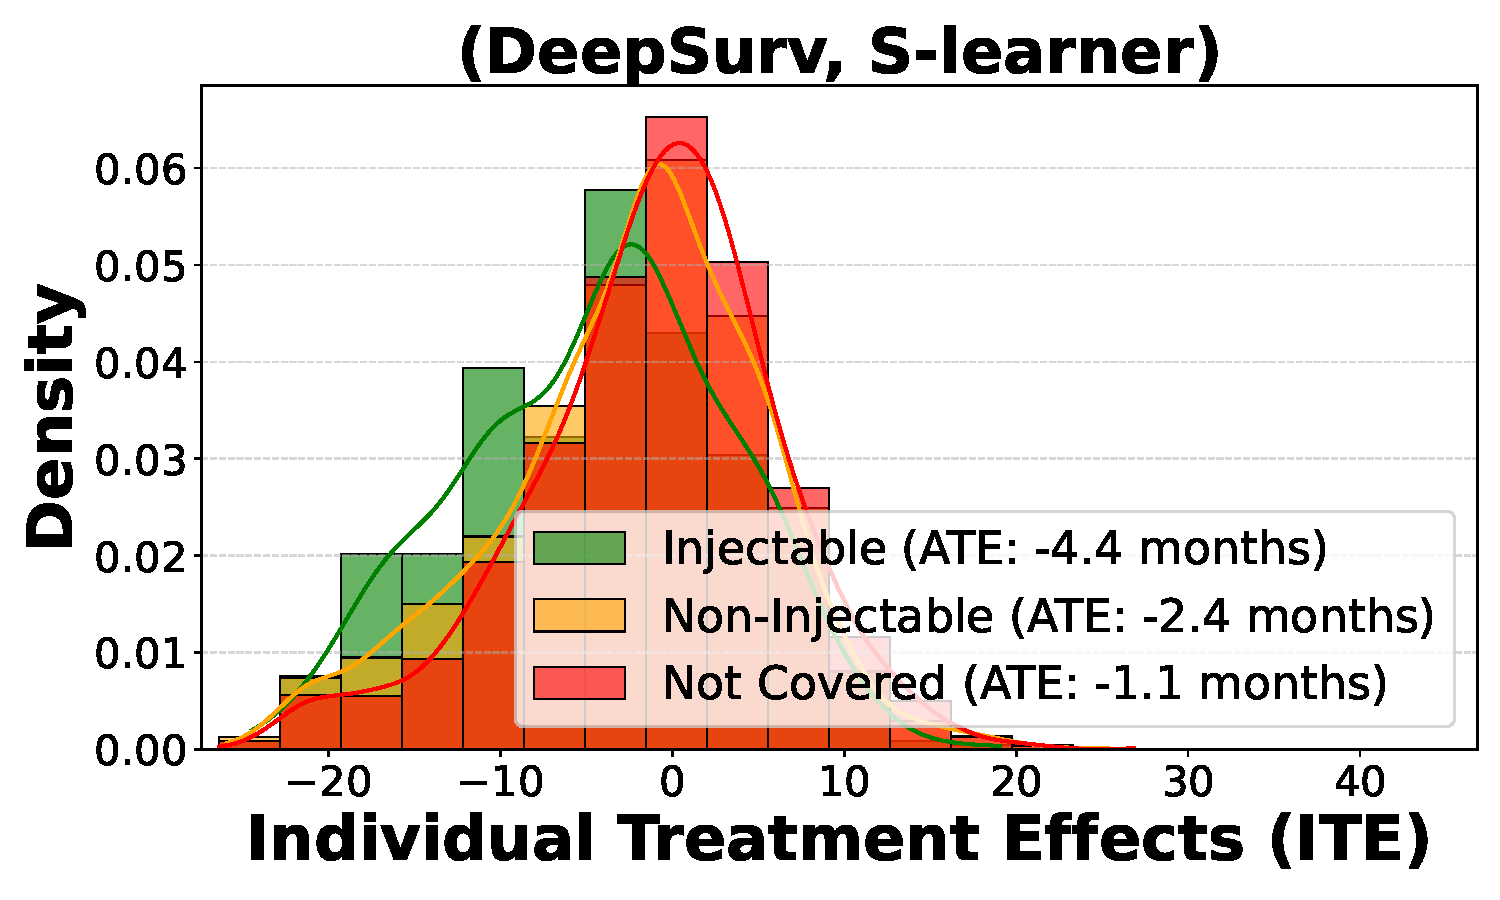
\includegraphics[width=.22\linewidth]{Appendices/appendix-ch03/images/ITE_injectable_full_3/ITE_DeepSurv_S-learner_injectable_type.pdf}}%
    \hfill
    \subfigure[\footnotesize (DeepSurv, Matching-1)]{\label{ch03:fig:ite_injectable_deepsurv_matching_1}%
      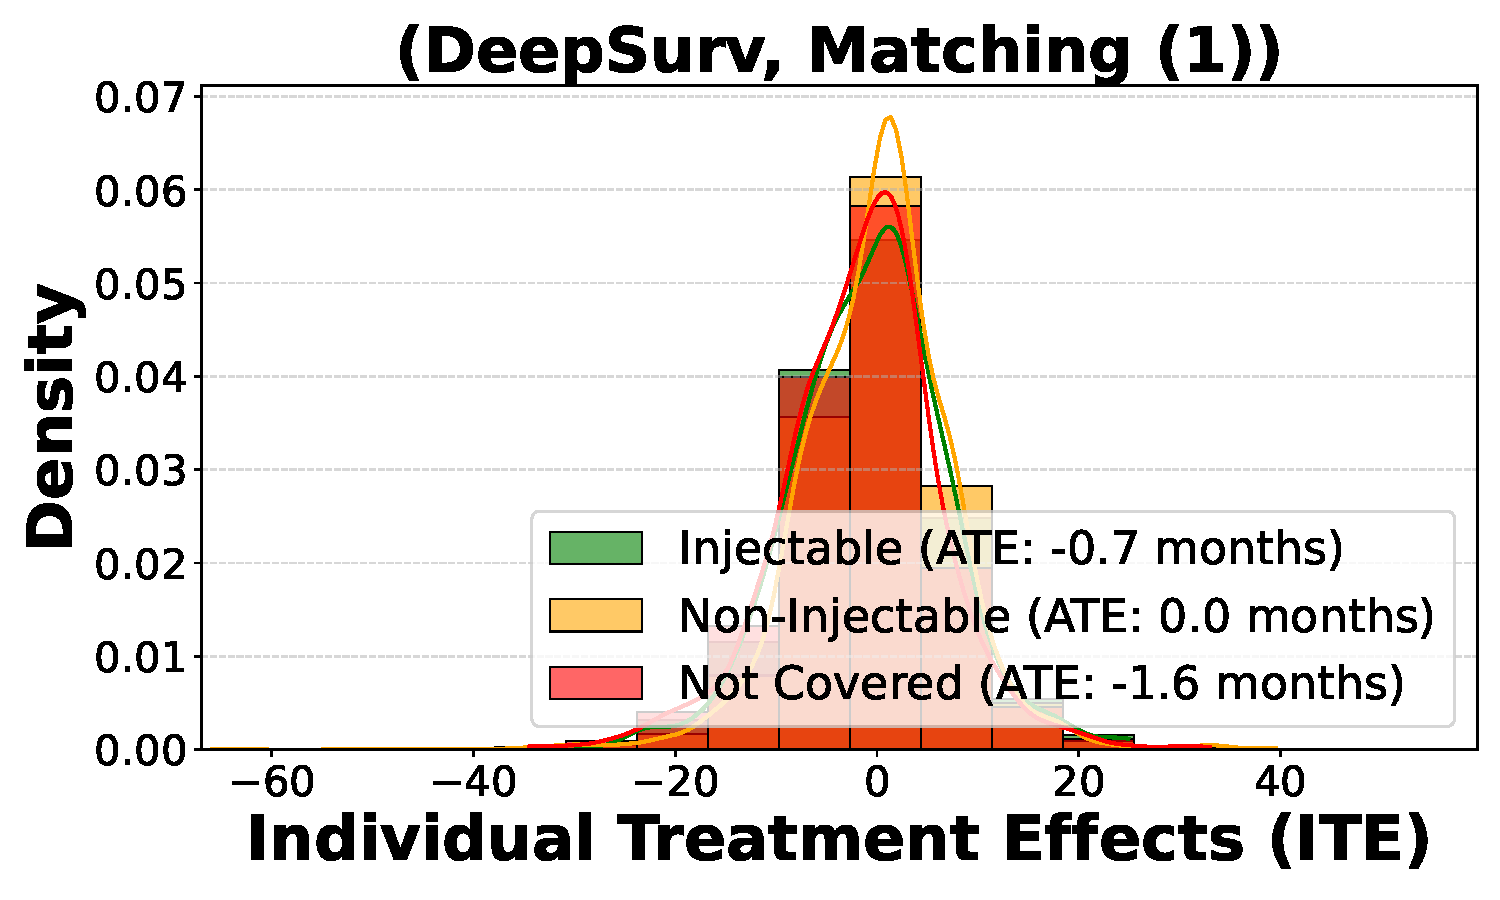
\includegraphics[width=.22\linewidth]{Appendices/appendix-ch03/images/ITE_injectable_full_3/ITE_DeepSurv_Matching_1_injectable_type.pdf}}%
    \hfill
    \subfigure[\footnotesize (DeepSurv, Matching-5)]{\label{ch03:fig:ite_injectable_deepsurv_matching_5}%
      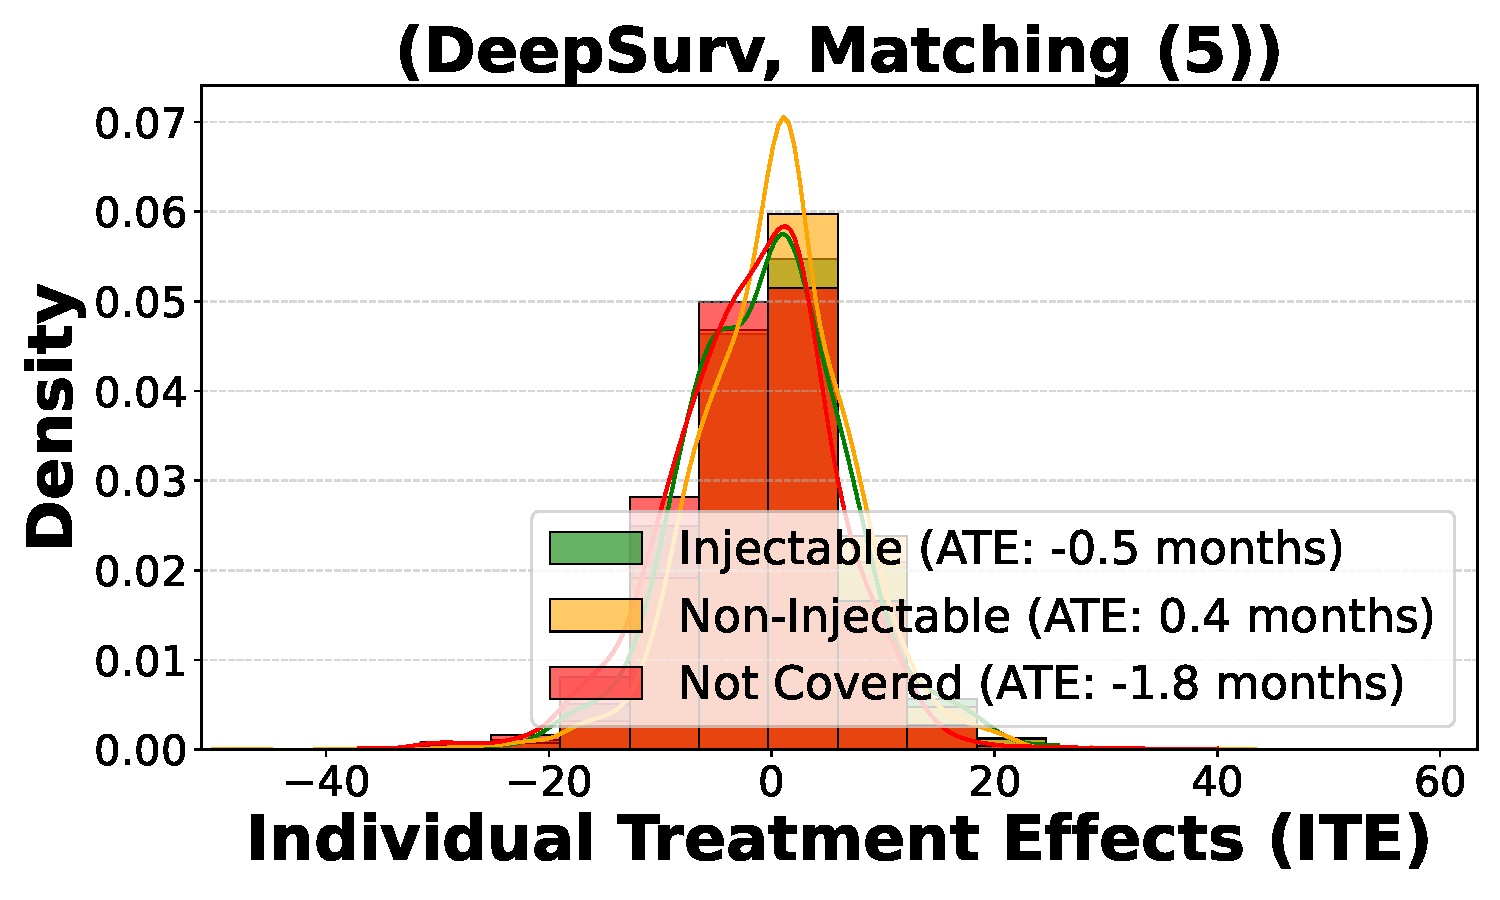
\includegraphics[width=.21\linewidth]{Appendices/appendix-ch03/images/ITE_injectable_full_3/ITE_DeepSurv_Matching_5_injectable_type.pdf}}%
    \\
    \subfigure[\footnotesize (RandomSurvivalForest, T-Learner)]{\label{ch03:fig:ite_injectable_rsf_t_learner}%
      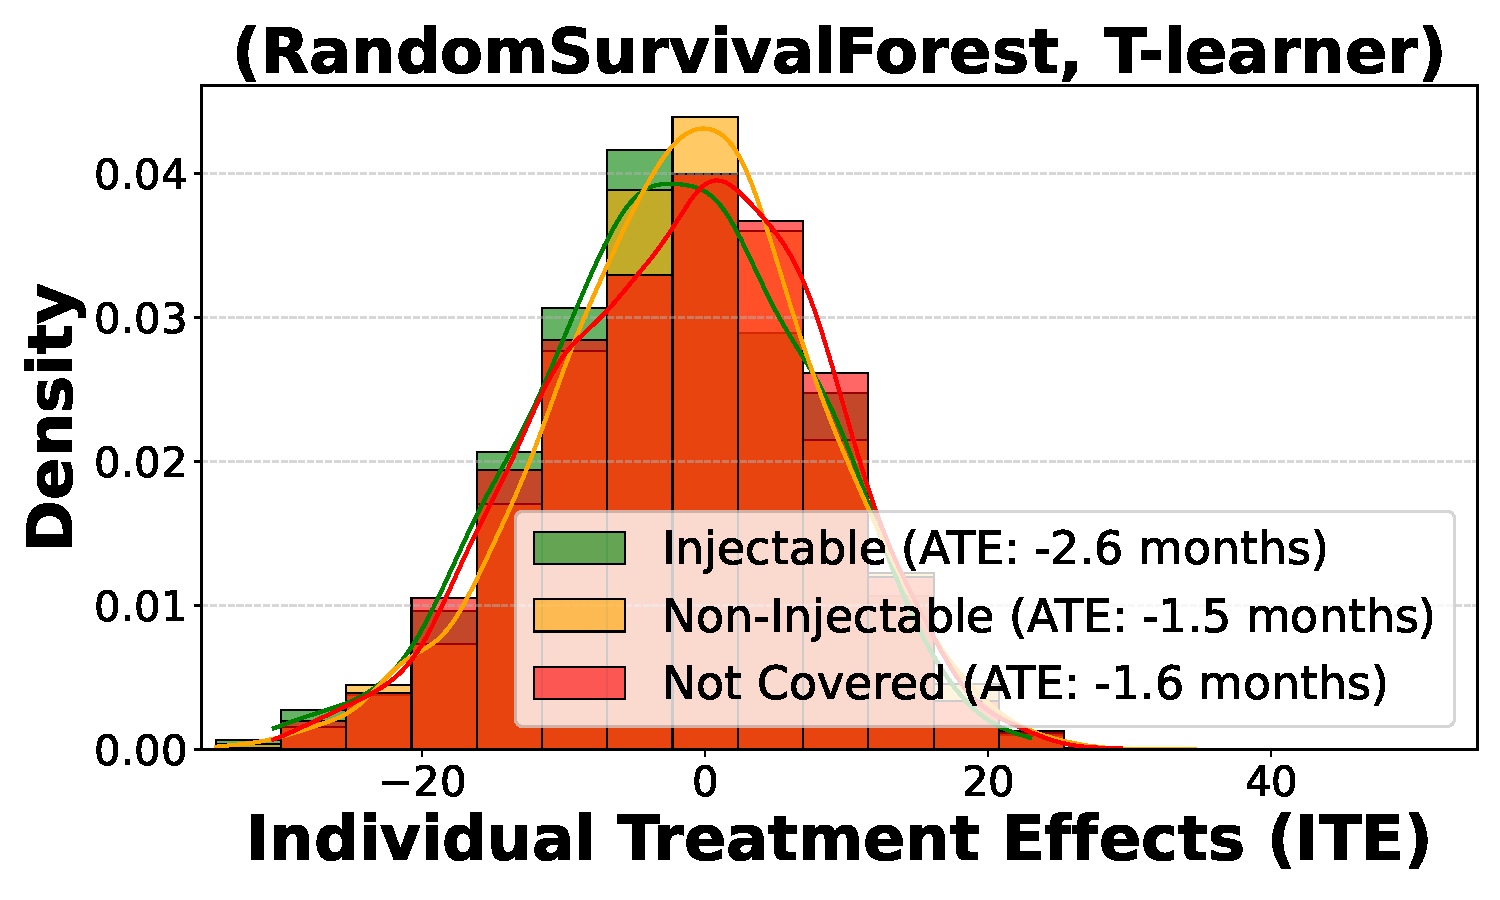
\includegraphics[width=.22\linewidth]{Appendices/appendix-ch03/images/ITE_injectable_full_3/ITE_RandomSurvivalForest_T-learner_injectable_type.pdf}}%
    \hfill
    \subfigure[\footnotesize (RandomSurvivalForest, S-Learner)]{\label{ch03:fig:ite_injectable_rsf_s_learner}%
      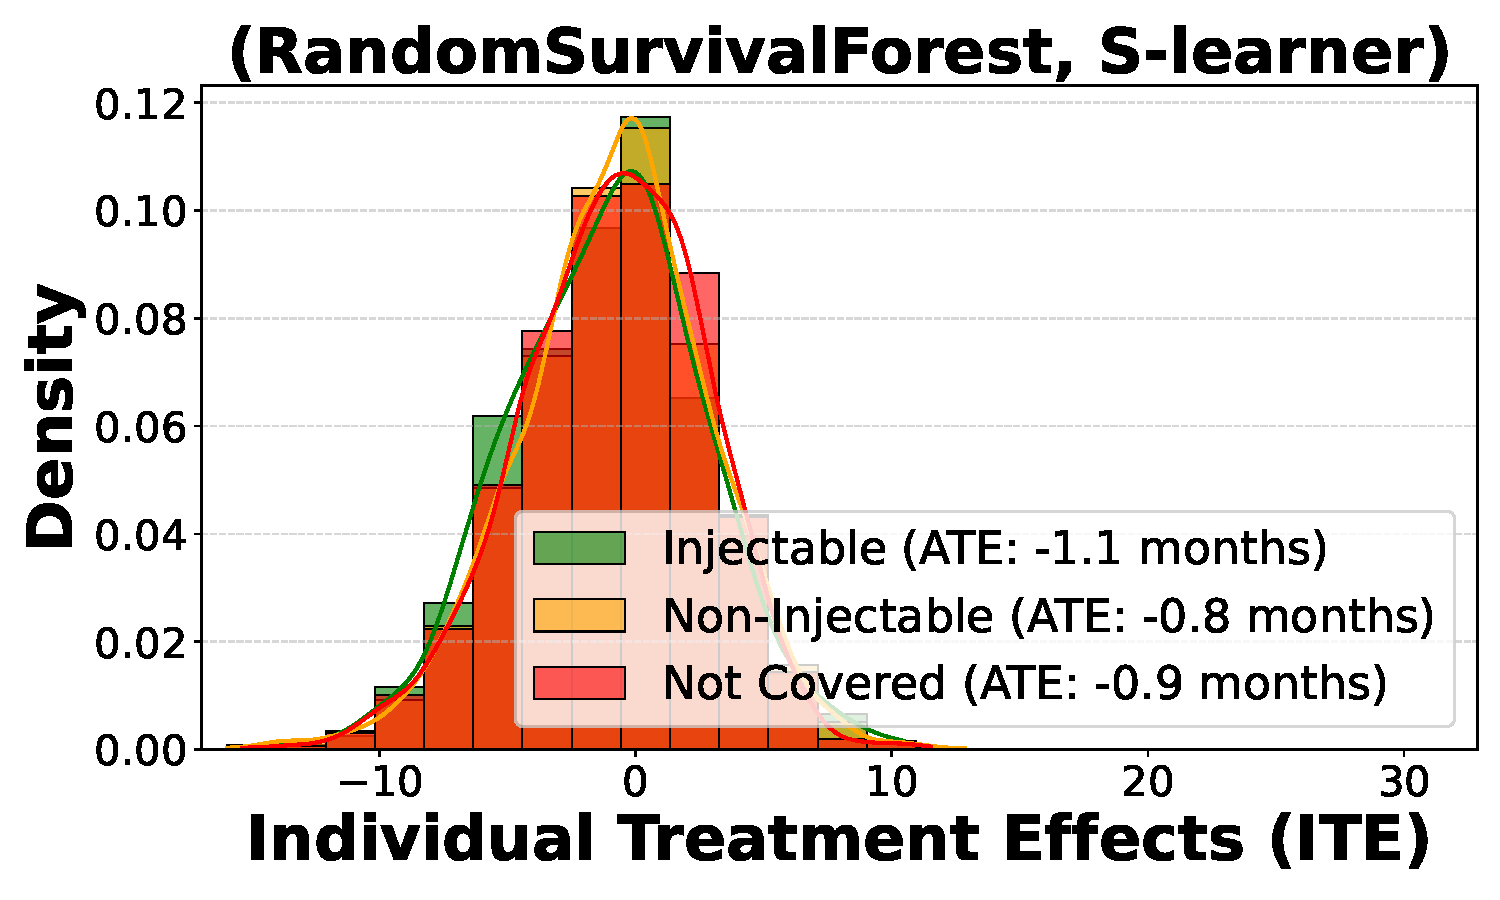
\includegraphics[width=.22\linewidth]{Appendices/appendix-ch03/images/ITE_injectable_full_3/ITE_RandomSurvivalForest_S-learner_injectable_type.pdf}}%
    \hfill
    \subfigure[\footnotesize (RandomSurvivalForest, Matching-1)]{\label{ch03:fig:ite_injectable_rsf_matching_1}%
      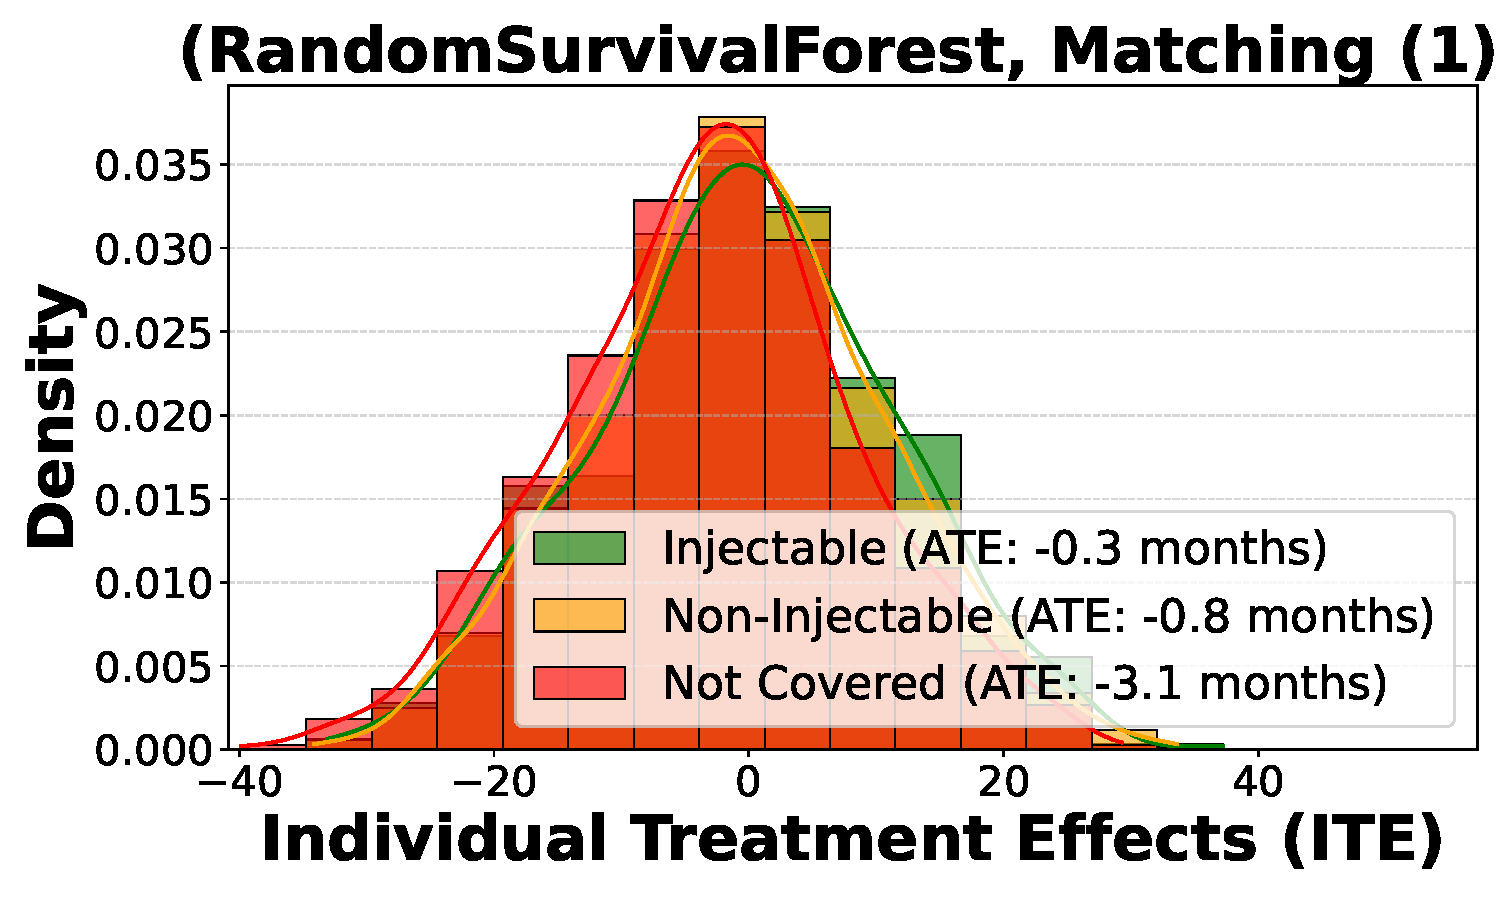
\includegraphics[width=.22\linewidth]{Appendices/appendix-ch03/images/ITE_injectable_full_3/ITE_RandomSurvivalForest_Matching_1_injectable_type.pdf}}%
    \hfill
    \subfigure[\footnotesize (RandomSurvivalForest, Matching-5)]{\label{ch03:fig:ite_injectable_rsf_matching_5}%
      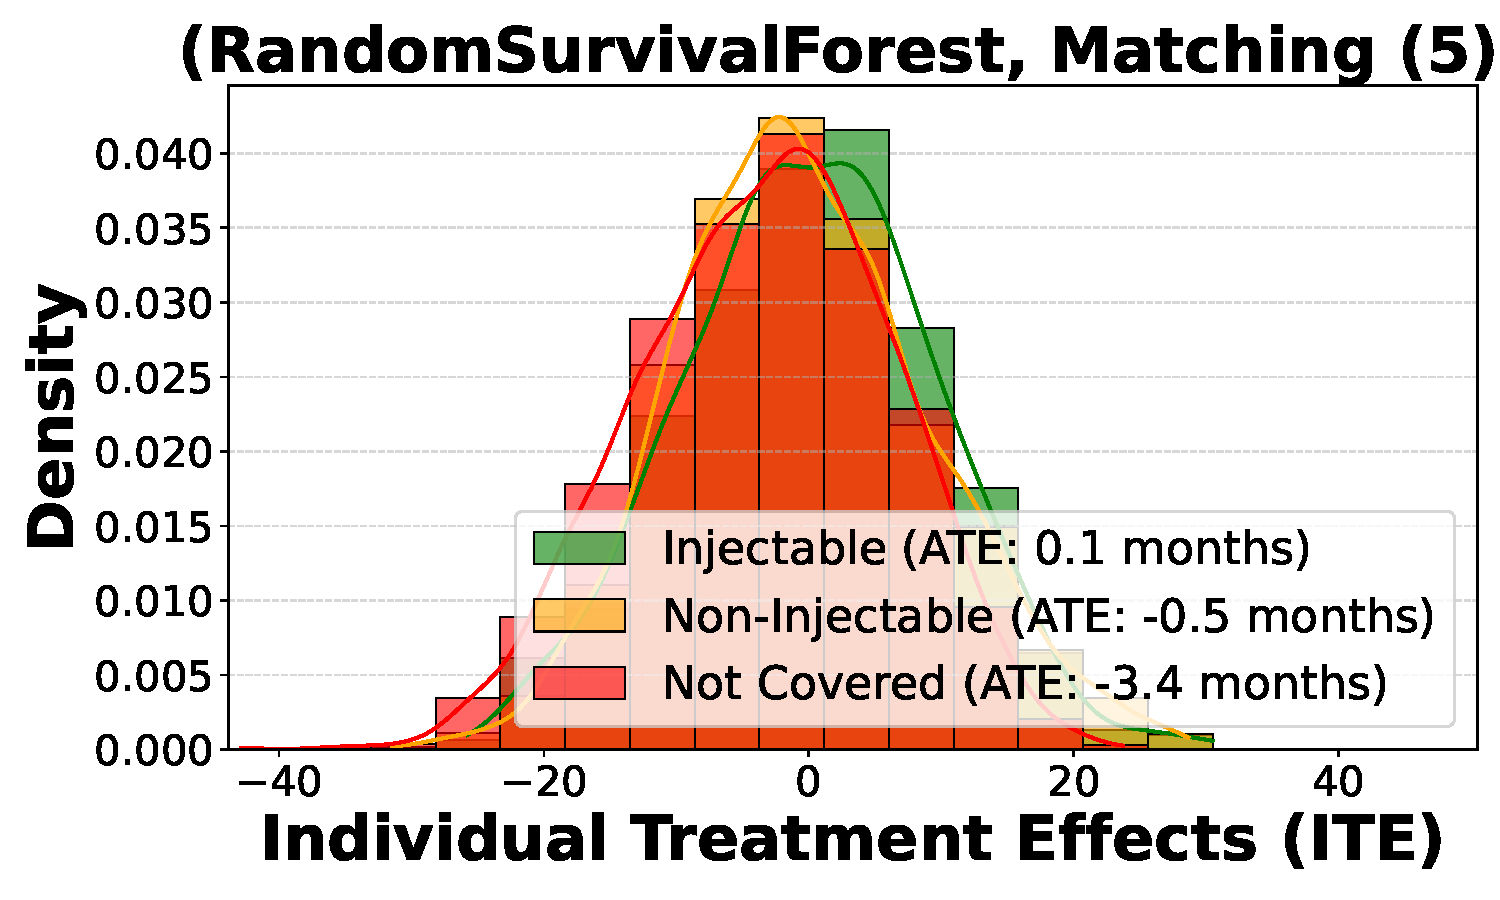
\includegraphics[width=.21\linewidth]{Appendices/appendix-ch03/images/ITE_injectable_full_3/ITE_RandomSurvivalForest_Matching_5_injectable_type.pdf}}%
    \\
    \subfigure[\footnotesize Causal Survival Forest]{\label{ch03:fig:ite_injectable_causal_survival_forest_all_3}%
      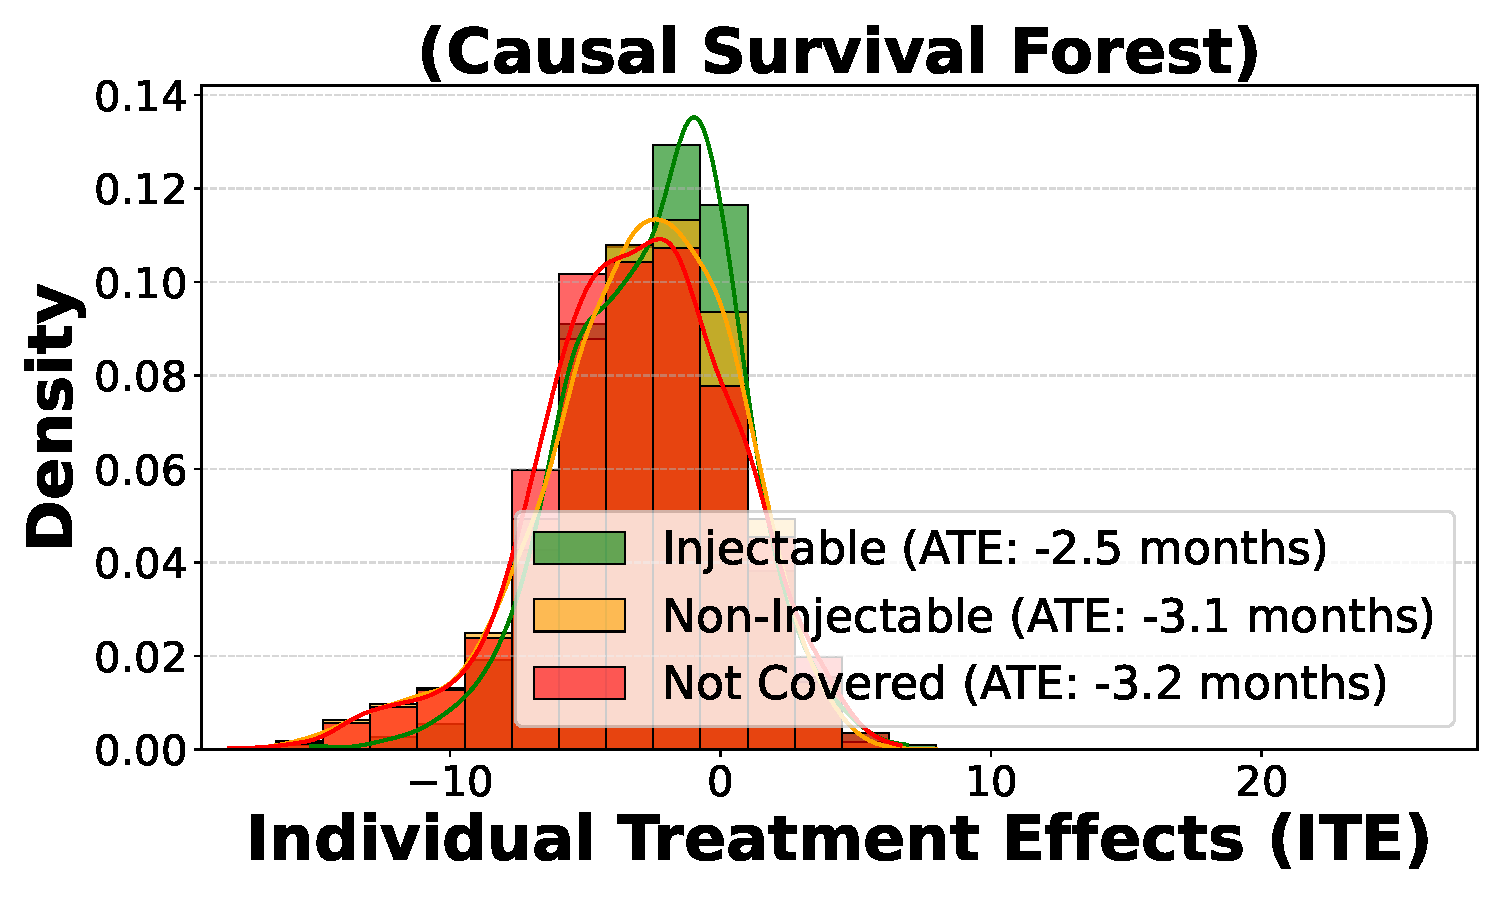
\includegraphics[width=.22\linewidth]{Appendices/appendix-ch03/images/ITE_injectable_full_3/ITE_CausalSurvivalForest_Causal_Survival_Forest_injectable_type.pdf}}
  }
\end{figure}


In this section, we present a detailed analysis of the Estimated Individual Treatment Effects (ITE) distributions across three medication adherence groups—injectable, non-injectable, and not covered—using various survival models and causal methods at the time snapshot \(\tau=3\) months.
Figure~\ref{ch03:fig:ite_injectable_all} provides a comprehensive view, with subfigures corresponding to different combinations of survival models (CoxPH, DeepSurv, Random Survival Forest) and causal inference approaches (T-learner, S-learner, and Matching methods with one and five matches) and an additional inherently causal survival model (Causal Survival Forest).

Across the survival models and causal methods, the Average Treatment Effect (ATE) values for injectable medications generally appear slightly more negative than those for non-injectable or not-covered groups.
This trend is most evident in the T-learner and S-learner approaches for CoxPH (Figures~\ref{ch03:fig:ite_injectable_coxph_t_learner}, \ref{ch03:fig:ite_injectable_coxph_s_learner}) and DeepSurv (Figures~\ref{ch03:fig:ite_injectable_deepsurv_t_learner}, \ref{ch03:fig:ite_injectable_deepsurv_s_learner}).
However, this distinction diminishes in Matching-based methods (Figures~\ref{ch03:fig:ite_injectable_coxph_matching_1}-\ref{ch03:fig:ite_injectable_coxph_matching_5} for CoxPH and Figures~\ref{ch03:fig:ite_injectable_deepsurv_matching_1}-\ref{ch03:fig:ite_injectable_deepsurv_matching_5} for DeepSurv), where the ATEs for injectables are closer to (and sometimes slightly less negative than) those for the non-injectable and not-covered groups.

The Causal Survival Forest (Figure~\ref{ch03:fig:ite_injectable_causal_survival_forest_all_3}) demonstrates a distinct pattern compared to other methods, with relatively narrower ITE distributions compared to most other models and less pronounced differences between adherence groups.
This consistency in ATE values across groups indicates minimal heterogeneity in treatment effects based on medication adherence formulation within this model.

Overall, the analysis suggests that while some survival models and causal methods reveal slight differences in ATEs for injectable medications, these differences are not substantial or consistent across methods.
The results align with the main findings reported in Section~\ref{ch03:sec:04_results_ite_analysis}, reinforcing the observation that the adherence effect on survival outcomes is largely uniform across injectable, non-injectable, and not-covered groups in the context of our dataset.
This lack of meaningful variability in ITEs suggests that medication formulation may not be a significant factor influencing adherence-related survival outcomes.
Future analyses could expand this approach to include additional adherence categories and explore whether patient subgroups or contextual factors contribute to heterogeneity in treatment effects.



